\documentclass[11pt,a4paper]{article}

% basic packages
\usepackage{float}
\usepackage{fullpage}
\usepackage{polski}
\usepackage{amsmath}
\usepackage{graphicx}
\usepackage[utf8x]{inputenc}

% bibliography and links
\usepackage{url}
\usepackage{cite}
\def\UrlBreaks{\do\/\do-}
\usepackage[hidelinks]{hyperref}

% graphs
\usepackage{tikz}
\usetikzlibrary{arrows}

% listings
\usepackage{listings}
\usepackage{color}
\definecolor{dkgreen}{rgb}{0,0.6,0}
\definecolor{gray}{rgb}{0.5,0.5,0.5}
\definecolor{mauve}{rgb}{0.58,0,0.82}
\lstset{
  basicstyle=\footnotesize,    
  captionpos=b,             
  commentstyle=\color{dkgreen},  
  frame=single,       
  keywordstyle=\color{blue},  
  language=Python,   
  numbers=left,     
  numbersep=7pt,   
  numberstyle=\tiny\color{gray}, 
  rulecolor=\color{black},  
  stringstyle=\color{mauve}, 
  tabsize=2,    
  title=\lstname
}

\begin{document}

\begin{titlepage}
  \begin{center}

    \textsc{\Large Politechnika Warszawska}\\[0.1cm]
    \small Wydział Elektroniki i Technik Informacyjnych
    \vfill

    \textsc{\small Grafy i Sieci}\\[0.1cm]
    \Huge Wyznaczanie klik w~grafie skierowanym\\[1.5cm]
    \small Sprawozdanie 3\\[2.5cm]

    \vfill

    \begin{minipage}{0.4\textwidth}
      \begin{flushleft} \large
        \emph{Autorzy:}\\[0.1cm]
        Maciej \textsc{Suchecki}\\
        Jacek \textsc{Witkowski}\\
      \end{flushleft}
    \end{minipage}
    \begin{minipage}{0.4\textwidth}
      \begin{flushright} \large
        \emph{Prowadzący:}\\[0.1cm]
        doc.~dr~inż.~Dariusz \textsc{Bursztynowski}\\[1cm]
      \end{flushright}
    \end{minipage}

    \vfill
    {\large \today}

  \end{center}
\end{titlepage}

\section{Część 1}
\subsection{Treść zadania}
\paragraph{Tytuł} Wyznaczanie klik w~grafie skierowanym
\paragraph{Opis} Wyznacz wszystkie kliki grafu skierowanego G. Wyjaśnienie: Kliką w grafie nieskierowanym G nazywamy każdy największy pełny podgraf G (w grafie pełnym każda para węzłów jest połączona krawędzią). Dla potrzeb projektu kliką grafu skierowanego G nazwiemy każdy największy pełny podgraf grafu G’ powstałego z G przez zastąpienie par krawędzi skierowanych (i→j), (j→i) krawędziami nieskierowanymi (i,j) i usunięcie krawędzi pozostałych. Problem znajdowania klik występuje m.in. w~optymalizacji szeregowania transmisji w radiowych sieciach wieloskokowych (ang. multihop).

\subsection{Implementacja}
\paragraph{Język programowania} Wybranym językiem programowania jest Java.
\paragraph{Założenia} Zakładamy, że graf wejściowy będzie skierowanym grafem spójnym.
\paragraph{Dane wejściowe} Dane wejściowe grafu będą w postaci listy krawędzi. Każda krawędź będzie reprezentowana w~nowej linii jako para uporządkowana (A, B), przy czym A będzie wierzchołkiem początkowym, a B wierzchołkiem docelowym.
\paragraph{Dane wyjściowe} Wynikiem działania programu będzie lista klik, przy czym każda klika będzie reprezentowana jako osobna linia składająca się z wierzchołków oddzielonych spacjami.

\newpage
\section{Część 2}
\subsection{Algorytm}
\subsubsection{Wybór}
Do rozwiązania problemu wybrany został algorytm rekurencyjny Brona-Kerboscha w~wersji z~piwotingiem oraz sortowaniem wierzchołków. Wybór jest uzasadniony wydajnością rozwiązania. Wersja z~piwotingiem charakteryzuje się zmniejszoną liczbą wywołań rekurencyjnych w~stosunku do wersji podstawowej algorytmu. Dodatkowo zastosowane zostało sortowanie wierzchołków, aby uzyskać lepszą klasę złożoności algorytmu.

\subsubsection{Pseudokod}
\begin{lstlisting}[mathescape = true, caption = Pseudokod algorytmu Brona-Kerboscha]
BronKerbosch(G):
  P = V(G)
  R = X = empty
  sort vertices in G
  for each vertex v in G:
    BronKerboschRecursive(R $\cup$ {v}, P $\cap$ N(v), X $\cap$ N(v))
    P := P $\setminus$ {v}
    X := X $\cup$ {v}

BronKerboschRecursive(R, P, X):
  if P is empty and X is empty:
    report R as a maximal clique
  choose a pivot vertex u in P $\cup$ X
  for each vertex v in P $\setminus$ N(u):
    BronKerbosch2(R $\cup$ {v}, P $\cap$ N(v), X $\cap$ N(v))
    P := P $\setminus$ {v}
    X := X $\cup$ {v}
\end{lstlisting}

\subsubsection{Opis}
Algorytm otrzymuje na wejściu graf G. Na początku tworzone są trzy zbiory P, R i X, przy czym: P to zbiór wierzchołków, które są kandydatami do rozważenia, R to zbiór wierzchołków będących częściowym wynikiem szukania kliki, a X to zbiór wierzchołków pominiętych. Przy pierwszym wywołaniu algorytmu zbiory R i X są puste, a zbiór P zawiera wszystkie wierzchołki grafu. Po zainicjalizowaniu zmiennych, wierzchołki grafu G są sortowane względem degeneracji, aby przyśpieszyć działanie algorytmu. Następnie dla każdego wierzchołka grafu wywoływana jest procedura rekurencyjna algorytmu, której zasada działania jest następująca:

\begin{enumerate}
  \item Najpierw sprawdzamy, czy zbiory P i X są puste. Jeśli tak, to zbiór R zawiera maksymalną klikę. Wypisujemy zawartość zbioru R i kończymy.
  \item Następnie wybieramy ze zbioru $P \cup X$ wierzchołek \textit{u}, który posłuży nam za \textit{pivot}.
  \item Ze zbioru P odejmujemy sąsiadów wierzchołka \textit{u}, tworząc nowy zbiór do badania w~pętli.
  \item Jeśli nowopowstały zbiór nie jest pusty, to wybieramy z niego kolejne wierzchołki v i~dla każdego z~nich:
    \begin{enumerate}
      \item Wywołujemy rekurencyjnie algorytm ze zbiorami R $\cup$ {v}, P $\cap$ N(v), X $\cap$ N(v).
      \item Ze zbioru P usuwamy wierzchołek v, dodając go jednocześnie do zbioru R.
    \end{enumerate}
\end{enumerate}

\paragraph{Opis zmiennych}
\begin{itemize}
  \item \textit{G} -- badany graf
  \item \textit{V(G)} -- zbiór wierzchołków badanego grafu
  \item \textit{P} -- zbiór wierzchołków, które są kandydatami do rozważenia
  \item \textit{R} -- zbiór wierzchołków będących częściowym wynikiem szukania kliki
  \item \textit{X} –- zbiór wierzchołków pominiętych
  \item \textit{v, u} –- zmienne pomocnicze przechowujące wierzchołki
  \item \textit{N(v)} -- zbiór sąsiadów wierzchołka v
\end{itemize}

\subsection{Opis struktur danych}
W programie graf jest reprezentowany jako zbiór krawędzi oraz zbiór węzłów (wierzchołków). Każda krawędź jest powiązana z dwoma węzłami. Każdy węzeł zawiera informację o etykiecie (unikalnej dla każdego węzła) oraz o swoich sąsiadach.

\subsection{Projekt testów}
Testy będą się odbywać w~dwóch etapach. Na początku zostanie przeprowadzona ręczna weryfikacja poprawności działania programu dla kilku prostych grafów wejściowych.\\

Ponadto, na potrzeby testów zakładamy napisanie skryptu w~języku Python, który będzie generował losowe grafy spełniające warunki zadania, uruchamiał program zbierając wyniki jego działania, a następnie wyświetlał wykresy obrazujące uzyskane wyniki. W ramach testów automatycznych zamierzamy otrzymać wykresy zależności czasu wykonania programu od liczby wierzchołków grafu oraz od jego gęstości.\\

Testy zakładają uśrednianie wyników dla kilku grafów o tych samych właściwościach (odpowiednio liczba wierzchołków oraz gęstość) dla zapewnienia wiarygodności wyników.

\subsection{Założenia programu}
\subsubsection{Złożoność obliczeniowa}
Pesymistyczna złożoność algorytmu Brona-Kerboscha (z~piwotingiem, który minimalizuje liczbę rekurencyjnych wywołań wykonanych w~każdym kroku) wynosi O($3^{n/3}$).\\

Natomiast wersja algorytmu z~sortowaniem wierzchołków -- wykorzystana w~programie -- osiąga złożoność O($dn3^{d/3}$), gdzie \textit{d} oznacza degenerację grafu, miarę jego rozproszenia. Zatem złożoność programu będzie liniowa względem liczby wierzchołków.

\subsubsection{Wejście}
\paragraph{Opis} Dane wejściowe do programu będą przekazywane w~postaci listy krawędzi grafu. Każda krawędź będzie reprezentowana w~nowej linii jako para uporządkowana (A, B), przy czym A będzie wierzchołkiem początkowym, a B wierzchołkiem docelowym.
\paragraph{Przykład} Dla grafu zdefiniowanego poniżej:\\

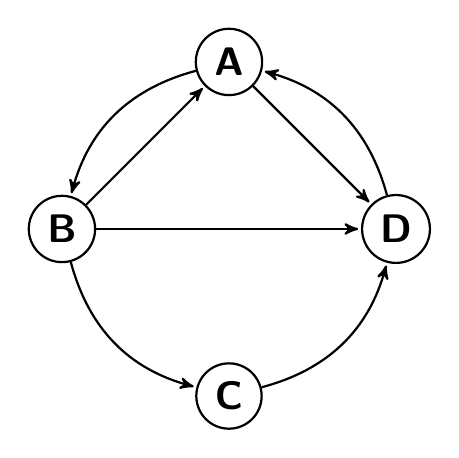
\begin{tikzpicture}[->,>=stealth',shorten >=1pt,auto,node distance=3cm,
  thick,main node/.style={circle,draw,font=\sffamily\Large\bfseries}]

  \node[main node] (1) {A};
  \node[main node] (2) [below left of=1] {B};
  \node[main node] (3) [below right of=2] {C};
  \node[main node] (4) [below right of=1] {D};

  \path[every node/.style={font=\sffamily\small}]
  (1) edge node [left] {} (4)
  edge [bend right] node[left] {} (2)
  (2) edge node [right] {} (1)
  edge node {} (4)
  edge [bend right] node[left] {} (3)
  (3) edge [bend right] node[right] {} (4)
  (4) edge [bend right] node[right] {} (1);
\end{tikzpicture}

\noindent Następujący plik wejściowy będzie uznany za poprawny:\\
\begin{lstlisting}[caption = Przykładowy plik wejściowy]
A B
A D
B A
B C
B D
C D
D A
\end{lstlisting}

\subsubsection{Wyjście}
\paragraph{Opis} Program będzie wypisywał w~kolejnych liniach listy wierzchołków stanowiące znalezione maksymalne kliki.
\paragraph{Przykład} Dla grafu zdefiniowanego poniżej:\\

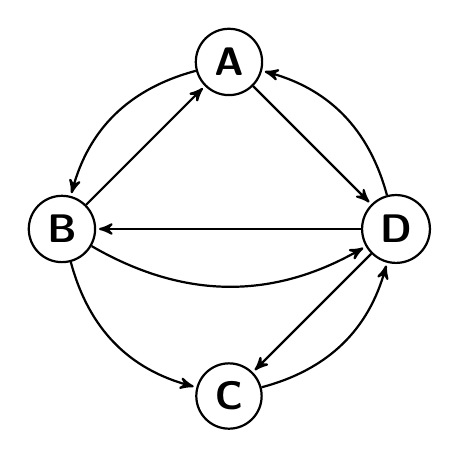
\begin{tikzpicture}[->,>=stealth',shorten >=1pt,auto,node distance=3cm,
  thick,main node/.style={circle,draw,font=\sffamily\Large\bfseries}]

  \node[main node] (1) {A};
  \node[main node] (2) [below left of=1] {B};
  \node[main node] (3) [below right of=2] {C};
  \node[main node] (4) [below right of=1] {D};

  \path[every node/.style={font=\sffamily\small}]
  (1) edge node [left] {} (4)
  edge [bend right] node[left] {} (2)
  (2) edge node [right] {} (1)
  edge [bend right] node {} (4)
  edge [bend right] node[left] {} (3)
  (3) edge [bend right] node[right] {} (4)
  (4) edge [bend right] node[right] {} (1)
  edge node {} (3)
  edge node {} (2);
\end{tikzpicture}

\noindent Program wygeneruje następujące wyjście:\\
\begin{lstlisting}[caption = Wynik działania programu]
A B D
D C
\end{lstlisting}

\section{Część 3}
W~ramach tej części projektu zostały stworzone testy algorytmu, sprawdzające zarówno jego poprawność, jak i~wydajność w~zależności od różnych czynników. Testy poprawności zostały wykonane w~języku Java, z~użyciem bibliotek: \textit{JUnit} oraz \textit{Mockito}. Z~kolei testy wydajnościowe zostały napisane w~języku skryptowym Python, z~wykorzystaniem bibliotek takich, jak: \textit{matplotlib} oraz \textit{numpy}. Generowanie grafów testowych zostało wykonane własnoręcznie, również w~języku Python. Testy te miały na celu wyznaczenie wydajności algorytmu w~zależności od trzech czynników:

\begin{itemize}
  \item rozmiaru grafu,
  \item gęstości grafu,
  \item degeneracji grafu.
\end{itemize}

Wyniki testowania algorytmu zostały przedstawione w~kolejnych sekcjach.

\subsection{Testy poprawności}
W celu sprawdzenia poprawności działania algorytmu wykonano dwa testy.
Pierwszy z nich miał na celu sprawdzić czy w zadanym grafie (rys. \textbf{TODO})
zostaną odnalezione odpowiednie kliki: (\textbf{TODO formatowanie}) 4,6,5; 0,1; 0,2; 0,3; 0,4;

Drugi z testów miał za zadanie sprawdzić czy algorytm sortowania
węzłów względem ich degeneracji działa zgodnie z oczekiwaniami.
W tym celu przygotowano graf (rys. \textbf{TODO}) i~spodziewano się!uzyskać
wierzchołki taką listę wierzchołków taką, że~na~początku tej~listy
znajdą się~wierzchołki o~numerach 1,2 i~3 (w~dowolnej kolejności), po~nich
wystąpi wierzchołek~0, a~po~nim wystąpią wierzchołki o~numerach 4,5 i 6.

Oba testy zakończyły się~powodzeniem.

\newpage
\subsection{Testy wydajnościowe}
W~ramach testów wydajnościowych zdecydowaliśmy się wykonać wykresy czasu działania algorytmu w~zależności od różnych czynników. W~tym celu używane są następujące funkcje napisane w~języku Python:\\

\begin{lstlisting}[caption = Funkcje pomocnicze dla testów wydajnoćiowych]
# runs the app with desired input graph
def runSolver(graphFilename):
  command = ["java", "-jar", "./GIS.jar", "-i", str(graphFilename)]
  result = subprocess.check_output(command)
  return result

# runs solver and records run time
def runSolverAndMeasureTime(graphFilename):
  start = timeit.default_timer()
  runSolver(graphFilename)
  stop = timeit.default_timer()
  time = stop - start
  return time

# runs solver multiple times with different graphs and collects average time
def collectAverageTime(graphFilenames):
  averageTime = 0
  for graph in graphFilenames:
    time = runSolverAndMeasureTime(graph)
    averageTime += time
  averageTime /= repetitions
  return averageTime

# plots a simple graph
def plotGraph(data, xlabel, ylabel):
  plot.plot(list(data.keys()), list(data.values()))
  plot.ylabel(ylabel)
  plot.xlabel(xlabel)
  plot.show()
\end{lstlisting}

Służą one odpowiednio do: uruchomienia algorytmu z~zadanym grafem, zmierzenia czasu jego wykonywania, uśredniania otrzymanych wyników oraz do rysowania wykresu na podstawie uzyskanych danych. Test dla każdego czynnika (rozmiaru, gęstości oraz degeneracji grafu) zakładają wykonanie następujących kroków:

\begin{enumerate}
  \item wyczyszczenie pamięci przechowującej rezultaty,
  \item dla każdej testowanej wartości parametru:
  \begin{enumerate}
    \item wygenerowanie 20 grafów o zadanych parametrach,
    \item uruchomienie algorytmu dla każdego z~wygenerowanych grafów,
    \item obliczenie średniej z~uzyskanych czasów wykonania,
    \item zapisanie średniej wraz z~testowaną wartością do pamięci.
  \end{enumerate}
  \item wyświetlenie wykresu.
\end{enumerate}

\newpage
\subsubsection{Generowanie grafów}
W~celu wygenerowania grafów testowych został napisany mały moduł w~języku Python, którego fragment zaprezentowany jest poniżej:
\begin{lstlisting}[caption = Funkcje generujące grafy dla testów wydajnościowych]
# generates random directed graph with desired number of vertices and density
def generateAndSaveGraphWithDesiredDensity(file, verticesCount, density):
  graphFile = open(file, "w")
  vertices = list(range(verticesCount))

  # calculate desired number of edges from desired graph density
  maxPossibleEdgeCount = verticesCount * (verticesCount - 1)
  edgeCount = int(density * maxPossibleEdgeCount)

  # generate random degrees in range [0, verticesCount-1] that sums to edgeCount
  degrees = generateDegrees(verticesCount, edgeCount, 0, verticesCount - 1)

  # generate dictionary containing vertex/degree pairs, then iterate over it,
  # drawing <degree> vertices from all possible ones and save edges to file
  for vertice, degree in dict(zip(vertices, degrees)).items():
    possibleSucc = list(vertices)
    possibleSucc.remove(vertice)     # avoid loops
    for successor in random.sample(possibleSucc, degree):
      graphFile.write(str(vertice) + " " + str(successor) + "\n")

  graphFile.close()

# generates random directed graph with desired number of vertices and degeneracy
def generateAndSaveGraphWithDesiredDegeneracy(file, verticesCount, degeneracy):
  graphFile = open(file, "w")
  vertices = list(range(verticesCount))
  possibleSucc = vertices

  # generate random degree in range [0, degeneracy] for every vertex to satisfy
  # degeneracy criterion (there should be at least 1 vertex with degree = deg.)
  degrees = [degeneracy]
  for _ in range(verticesCount - 1):
    degrees.append(random.randint(0, degeneracy))
  degrees.sort(reverse=True)

  # for every vertice, generate random number of its successors (less than
  # degeneracy), then take that number of vertices from successors set and save
  # resulting pairs to file with desired filename as two-way edges;
  # from the rest, draw a random number to generate one-way edges
  for vertice, degree in dict(zip(vertices, degrees)).items():
    possibleSucc.remove(vertice)     # prevent loops and duplicate edges
    twoWaySucc = random.sample(possibleSucc, min(degree, len(possibleSucc)))
    oneWaySucc = [item for item in possibleSucc if item not in twoWaySucc]

    # generate two way edges
    for successor in twoWaySucc:
      graphFile.write(str(vertice) + " " + str(successor) + "\n")
      graphFile.write(str(successor) + " " + str(vertice) + "\n")

    # generate couple random one-way edges
    for successor in random.sample(oneWaySucc, random.randint(0, len(oneWaySucc))):
      graphFile.write(str(vertice) + " " + str(successor) + "\n")

  graphFile.close()
\end{lstlisting}

\newpage
\subsubsection{Wydajność w~zależności od rozmiaru grafu}
Dla wykonania testów wydajności w~funkcji rozmiaru grafu, uruchomiono następujący kod:\\

\begin{lstlisting}[caption = Testy wydajności w~zależności od rozmiaru grafu]
results = {}
for size in sizes:
  graphFilenames = graph.generateRandomGraphs(count, size)
  results[size] = collectAverageTime(graphFilenames)
plotGraph(results, "Rozmiar grafu (liczba wierzcholkow)", "Czas wykonywania (ms)")
\end{lstlisting}

W~wyniku jego działania uzyskano następujący wykres:

\begin{figure}[H]
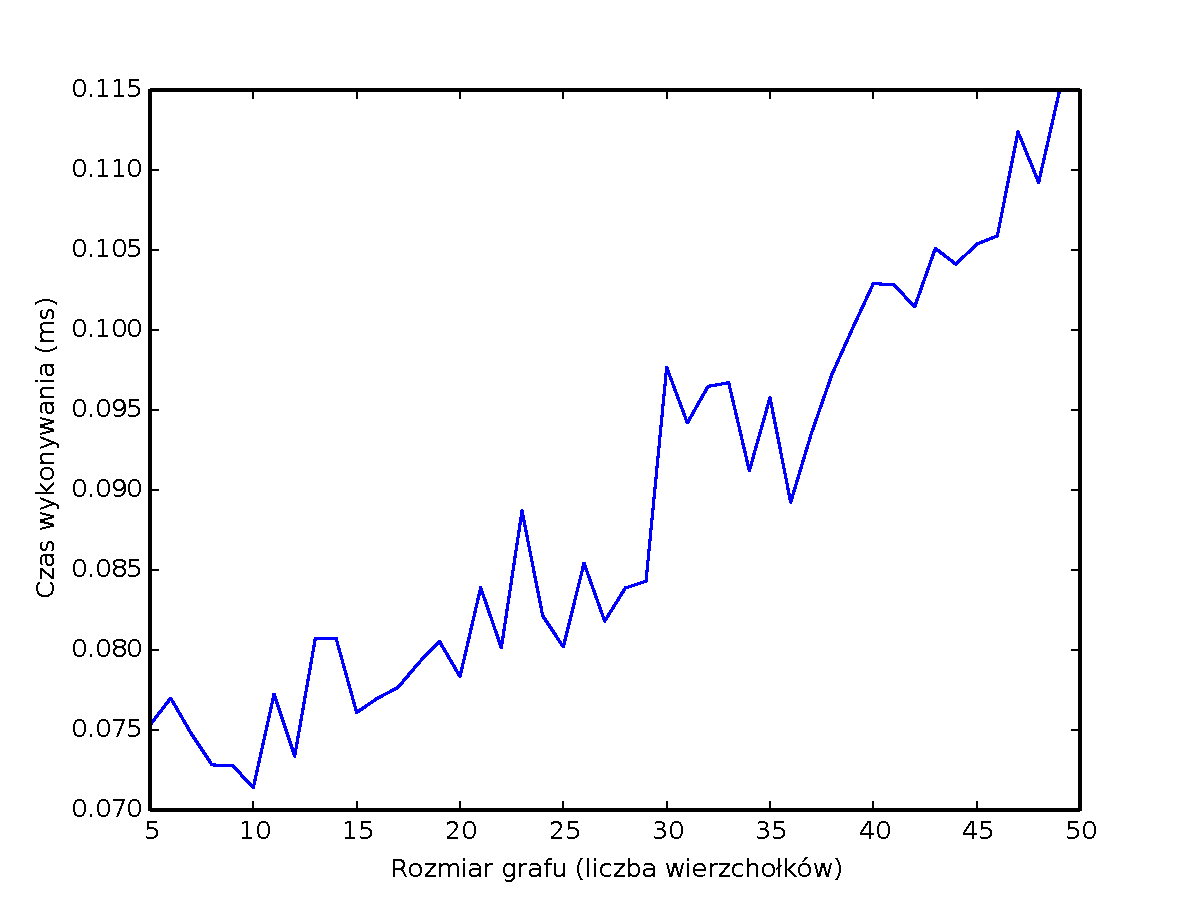
\includegraphics[trim = 0mm 2mm 0mm 12mm, clip, width=14cm]{img/size.pdf}
\caption{Wpływ rozmiaru grafu na wydajność algorytmu.}
\end{figure}

Po przeanalizowaniu wykresu widoczny jest oczywiście wyraźny wzrost czasu wykonywania algorytmu podczas wzrostu rozmiaru grafu. Po dokładnym przyjrzeniu się kształtowi otrzymanego wykresu, można zaryzykować stwierdzenie, że złożoność algorytmu jest liniowa w~zależności od rozmiaru grafu.

\newpage
\subsubsection{Wydajność w~zależności od gęstości grafu}
Dla wykonania testów wydajności w~funkcji gęstości grafu, uruchomiono następujący kod:\\

\begin{lstlisting}[caption = Testy wydajności w~zależności od gęstości grafu]
results = {}
for density in densities:
  graphFilenames = graph.generateRandomGraphsWithDensity(count, size, density)
  results[size] = collectAverageTime(graphFilenames)
plotGraph(results,
          "Gestosc grafu (liczba krawedzi / najwieksza mozliwa liczba krawedzi)",
          "Czas wykonywania (ms)")
\end{lstlisting}

W~wyniku jego działania uzyskano następujący wykres:

\begin{figure}[H]
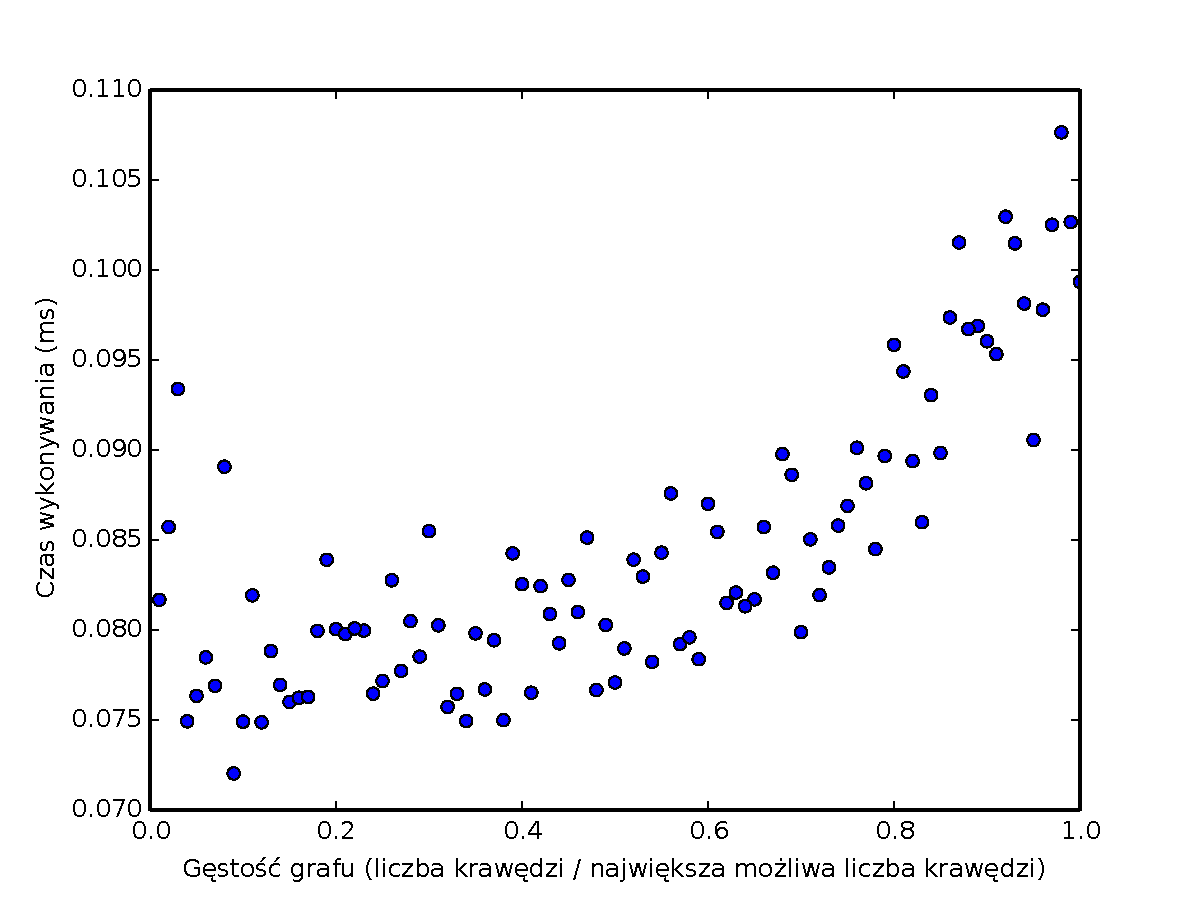
\includegraphics[trim = 0mm 2mm 0mm 12mm, clip, width=14cm]{img/density.pdf}
\caption{Wpływ gęstości grafu na wydajność algorytmu.}
\end{figure}

Na wykresie nie zauważyliśmy wyraźnej i~jednocześnie jednoznacznej zależności wydajności algorytmu w~funkcji gęstości testowanego grafu. Można oczywiście zauważyć wyraźny wzrost czasu wykonywania algorytmu podczas wzrostu gęstości grafu, jednakże trudno tu o~jednoznaczne stwierdzenie złożoności wykładniczej z~racji na dość duży rozrzut uzyskiwanych wyników (pomimo ich uśredniania).

\newpage
\subsubsection{Wydajność w~zależności od degeneracji grafu}
Z powodu niezauważenia przez nas wyraźnej i~jednoznacznej zależności wydajności algorytmu od gęstości grafu, zdecydowaliśmy się na wykonanie wykresu w~zależności od degeneracji grafu. Dla wykonania testów wydajności w~funkcji rozmiaru grafu, uruchomiono następujący kod:\\

\begin{lstlisting}[caption = Testy wydajności w~zależności od degeneracji grafu]
results = {}
for degeneracy in degeneracies:
  graphFilenames =
    graph.generateRandomGraphsWithDegeneracy(count, size, degeneracy)
  results[degeneracy] = collectAverageTime(graphFilenames)
plotGraph(results, "Degeneracja grafu", "Czas wykonywania (ms)")
\end{lstlisting}

W~wyniku jego działania uzyskano następujący wykres:

\begin{figure}[H]
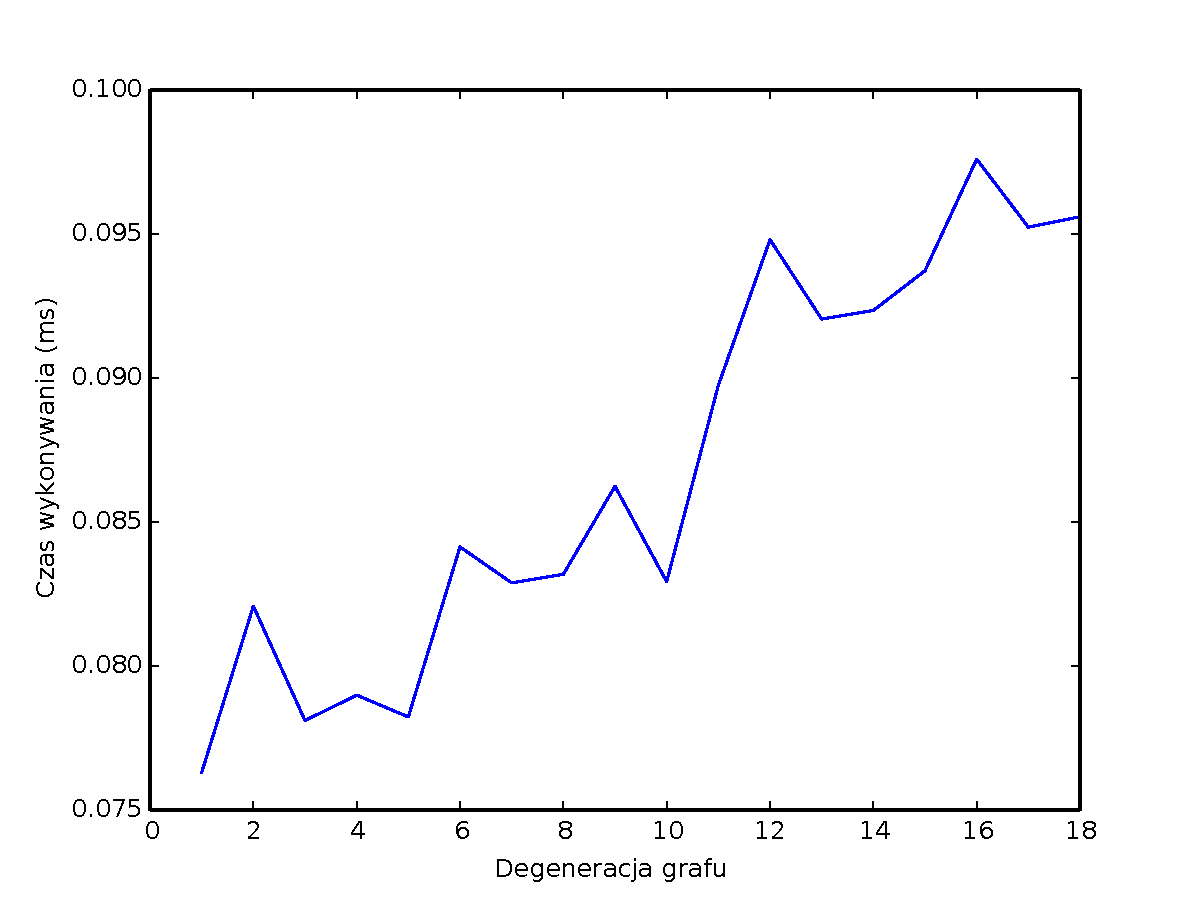
\includegraphics[trim = 0mm 2mm 0mm 12mm, clip, width=14cm]{img/degeneracy.pdf}
\caption{Wpływ degeneracji grafu na wydajność algorytmu.}
\end{figure}

Jak widać, wyniki są zgodne z~założeniami teoretycznymi nt. algorytmu -- złożoność algorytmu w~zależności od degeneracji grafu jest wykładnicza.

\end{document}
